% SynapSense one-page summary, IEEE conference style.
% Build:  cd docs/ieee && python make_figures.py && tectonic synapsense_ieee.tex
\documentclass[conference,letterpaper,9pt]{IEEEtran}
\usepackage[T1]{fontenc}
\usepackage{newtxtext,newtxmath}  % Times, as in IEEE templates
\usepackage{amsmath}
\usepackage{graphicx}
\usepackage{xcolor}
\usepackage{url}
\usepackage{cite}

\newcommand{\dps}{$^\circ$/s}
\setlength{\floatsep}{6pt plus 2pt minus 2pt}
\setlength{\textfloatsep}{8pt plus 2pt minus 2pt}

\begin{document}
% tighter space around the two equations
\setlength{\abovedisplayskip}{3pt plus 1pt}\setlength{\belowdisplayskip}{3pt plus 1pt}

\title{SynapSense: A Wrist-Worn Seizure Alert}

\author{\IEEEauthorblockN{Enes Sissenbi, Ivan Ni, Danish Puri}
\IEEEauthorblockA{Embedded Challenge, Fall 2026 \quad\textit{Educational prototype}}}

\IEEEaftertitletext{\vspace{-1.5\baselineskip}}
\maketitle

\begin{abstract}
SynapSense is a wrist-worn prototype that detects the convulsive phase of tonic--clonic seizures and alerts a paired
phone over Bluetooth Low Energy (BLE). Its rule-based IMU classifier stayed quiet in everyday wear and alerted
18\,s into a simulated convulsion.
\end{abstract}

\section{What It Detects}
Tonic--clonic seizures cause sustained, rhythmic limb jerking~\cite{cdc,ef,ilae}, and wrist motion sensing is the
best-supported noninvasive way to detect them~\cite{aes,meta}. SynapSense targets that clonic
phase: \emph{strong, regular 2--8\,Hz arm jerking with wrist rotation, for about 8\,s or more}. It does not detect absence, focal-aware, atonic or other low-motion seizures, warn before the
convulsion or diagnose epilepsy.

\section{System Design}
The XIAO nRF52840 Sense (LSM6DS3TR-C IMU) and a 90\,mAh LiPo sit in a 3D-printed case on a 19\,mm strap
(Fig.~\ref{fig:main}a--b); firmware is Arduino on PlatformIO. The IMU's FIFO buffers accelerometer ($\pm$8\,g) and
gyroscope ($\pm$2000\,\dps) samples at 52\,Hz and interrupts once a second; the MCU sleeps (FreeRTOS tickless
idle) in between. A RAM ring buffer holds the last 30\,s of raw data, frozen as a snapshot at every alert.
Power savers: FFT once a second, gyro in normal mode, microphone off, slower BLE advertising after 30\,s.

\section{Detection Algorithm}
After a 0.5-Hz high-pass filter, each 4-s window (recomputed every second; 256-point FFT, three axes' spectra
summed) gives, for accelerometer ($a$) and gyroscope ($\omega$), the RMS, dominant frequency $f$ and rhythm $\rho$: the
share of 0.6--15\,Hz power at the peak and its second harmonic. A window is a \emph{candidate} when
\begin{equation}
\begin{aligned}
c ={} & [a_{\mathrm{rms}} \ge 0.3\,\mathrm{g}] \land [\omega_{\mathrm{rms}} \ge 100\,^\circ\!/\mathrm{s}]\\
& \land [f_a, f_\omega \in [2,8]\,\mathrm{Hz}] \land [\rho_a, \rho_\omega \ge 0.3]
\end{aligned}
\end{equation}
and the newest second alone reaches 70\% of both RMS limits. Eight candidates in the last ten windows start a
PRE-ALERT; with no cancel, the ALERT follows 10\,s later with confidence
\begin{equation}
C = 100\left(0.6\,\tfrac{n}{10} + 0.4\min\!\left(1, \tfrac{\bar\rho}{0.6}\right)\right)\%,
\end{equation}
where $n$ is the candidate count and $\bar\rho$ their mean rhythm. Updates follow every 30\,s; ENDED is sent after
15\,s without rhythm (looser thresholds: hysteresis), then a 60-s cooldown: one alert per seizure.

\section{Avoiding False Alarms}
\begin{figure}[t]
\centering
\setlength{\fboxsep}{1pt}
\newcommand{\photo}[2]{\includegraphics[width=0.493\columnwidth]{#1}%
  \llap{\makebox[0.493\columnwidth][l]{\hspace{3pt}\raisebox{3pt}{\colorbox{white}{\footnotesize #2}}}}}
\photo{photo_top.jpg}{(a)}\hfill\photo{photo_side.jpg}{(b)}\\[3pt]
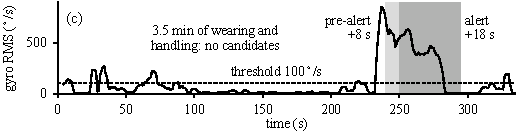
\includegraphics[width=\columnwidth]{fig_recording.pdf}
\caption{(a) Top and (b) side view (34$\times$25$\times$20.5\,mm case, USB-C port on the side). (c) Wrist
recording replayed through the detector; shading: pre-alert, then alert.}
\label{fig:main}
\end{figure}
\emph{Several features at once:} walking and running arm swing (1--1.5\,Hz) fails the band test, tooth brushing and
clapping fail the rotation or rhythm test, and brief bursts such as waving fail the 8-of-10 test. \emph{Two-stage
alert:} a double-tap (the IMU's tap engine) cancels a pre-alert only while the wrist is steady, since clonic jerks can
resemble taps and a seizure must never cancel its own alert; no response means the alert is sent. \emph{Faults kept
apart:} IMU failure, FIFO overrun, clipping and low battery go to a separate Status channel.

\section{Using the Device}
Wear it snug and charge it over USB-C (about 2\,h). In nRF Connect, connect to \textsf{SynapSense}, subscribe to
Alert and Status (as text) in service \texttt{7A3E0001-\ldots}, and write \texttt{test}, \texttt{cancel},
\texttt{ack} or \texttt{status} to Command. LED signals are in Table~\ref{tab:led}.

\begin{table}[t]
\caption{LED Signals}
\label{tab:led}
\centering
\footnotesize
\begin{tabular}{@{}p{0.36\columnwidth}p{0.59\columnwidth}@{}}
\hline
\textbf{Pattern} & \textbf{Meaning}\\
\hline
Blue / green blip every 5\,s & on; phone not connected / connected\\
Amber blinking & pre-alert: hold still, double-tap to cancel\\
Fast red blinking & alert sent to the phone\\
Red blip every 3\,s & alert not yet acknowledged\\
Long green & cancelled or acknowledged\\
3 quick red & cancel ignored: wrist still moving\\
Purple double blink & sensor fault\\
\hline
\end{tabular}
\end{table}

\section{Evaluation and Limits}
A real wrist recording replayed on a PC gives the same events as the board (Fig.~\ref{fig:main}c): 3.5\,min of
wearing and handling gave no candidates, and a 48-s forearm shake at 4--6\,Hz gave a pre-alert after 8\,s and one
alert (94\% confidence) after 18\,s. Limits:
thresholds come from simulated shaking, not clinical data; vigorous rhythmic activity can cause a (cancellable)
pre-alert; only a connected phone gets alerts.

\begin{thebibliography}{5}
\bibitem{cdc} CDC, ``Types of seizures,'' May 2024. [Online].
Available: \url{https://www.cdc.gov/epilepsy/about/types-of-seizures.html}
\bibitem{ef} Epilepsy Foundation, ``Types of seizures.'' [Online]. Available:
\url{https://www.epilepsy.com/what-is-epilepsy/seizure-types}
\bibitem{ilae} ILAE, ``Updated classification of epileptic seizures:
Position paper.'' [Online]. Available: \url{https://pmc.ncbi.nlm.nih.gov/articles/PMC12169392/}
\bibitem{aes} American Epilepsy Society, Epilepsy Foundation, and Danny Did Foundation, ``Position statement
on noninvasive seizure detection/alerting devices.'' [Online]. Available:
\url{https://cms.aesnet.org/about/about-aes/position-statements/noninvasive-seizure-detection-alerting-devices}
\bibitem{meta} ``Automated seizure detection using wearable devices: Updated systematic review and
meta-analysis,'' 2026. [Online]. Available: \url{https://pmc.ncbi.nlm.nih.gov/articles/PMC13350324/}
\end{thebibliography}

\end{document}
